\documentclass[12pt,a4paper]{report}
\usepackage{graphicx}
\usepackage{hyperref}
\usepackage{listings}
\usepackage{xcolor}
\usepackage{geometry}
\usepackage{titlesec}
\usepackage{fancyhdr}
\usepackage{atbegshi}
\usepackage{background}
\usepackage{tikz}
\usetikzlibrary{shapes,arrows,calc,positioning,fit}
\usepackage{forest}

% Define custom border style
\backgroundsetup{
  scale=1,
  angle=0,
  opacity=1,
  contents={
    
\begin{tikzpicture}[remember picture, overlay]
      \draw [line width=1pt, black]
        ($(current page.north west) + (1cm,-1cm)$)
        rectangle
        ($(current page.south east) + (-1cm,1cm)$);
    \end{tikzpicture}
  }
}

% Add this line to apply the page border to every page
\geometry{a4paper, margin=1in}

% Title formatting
\titleformat{\chapter}[display]
{\normalfont\huge\bfseries}{\chaptertitlename\ \thechapter}{20pt}{\Huge}
\titlespacing*{\chapter}{0pt}{50pt}{40pt}

% Code listing style
\lstset{
    basicstyle=\ttfamily\small,
    breaklines=true,
    commentstyle=\color{green!50!black},
    keywordstyle=\color{blue},
    stringstyle=\color{red},
    numbers=left,
    numberstyle=\tiny\color{gray},
    numbersep=5pt,
    frame=single,
    framexleftmargin=15pt,
    framexrightmargin=0pt,
    framexbottommargin=5pt,
    framextopmargin=5pt,
    backgroundcolor=\color{gray!10},
    showstringspaces=false
}

\lstdefinelanguage{JavaScript}{
  keywords={typeof, new, true, false, catch, function, return, null, catch, switch, var, if, in, while, do, else, case, break},
  keywordstyle=\color{blue}\bfseries,
  ndkeywords={class, export, boolean, throw, implements, import, this},
  ndkeywordstyle=\color{darkgray}\bfseries,
  identifierstyle=\color{black},
  sensitive=false,
  comment=[l]{//},
  morecomment=[s]{/}{/},
  commentstyle=\color{purple}\ttfamily,
  stringstyle=\color{red}\ttfamily,
  morestring=[b]',
  morestring=[b]'
}

\lstdefinelanguage{TypeScript}{
  keywords={typeof, new, true, false, catch, function, return, null, catch, switch, var, if, in, while, do, else, case, break},
  keywordstyle=\color{blue}\bfseries,
  ndkeywords={class, export, boolean, throw, implements, import, this},
  ndkeywordstyle=\color{darkgray}\bfseries,
  identifierstyle=\color{black},
  sensitive=false,
  comment=[l]{//},
  morecomment=[s]{/}{/},
  commentstyle=\color{purple}\ttfamily,
  stringstyle=\color{red}\ttfamily,
  morestring=[b]',
  morestring=[b]'
}

\renewcommand{\headrulewidth}{0.4pt}
\renewcommand{\footrulewidth}{0.4pt}

\pagestyle{fancy}
\fancyhf{}
\fancyhead[R]{E-Banking System}
\fancyfoot[C]{\thepage}

\begin{document}

\begin{titlepage}
    \centering
    \vspace*{1cm}
    {\huge\bfseries WEB-TECHNOLOGIES PROJECT REPORT\par}
    \vspace{1cm}
    {\Large\bfseries on\par}
    \vspace{1cm}
    {\huge\bfseries E-BANKING SYSTEM\par}
    \vspace{2cm}
    {\Large\bfseries Bachelor of Technology\par}
    \vspace{0.5cm}
    {\Large\bfseries In\par}
    \vspace{0.5cm}
    {\Large\bfseries Computer Science and Engineering\par}
    \vspace{2cm}
    {\Large\bfseries Under esteemed Guidance of\par}
    \vspace{0.5cm}
    {\Large\bfseries Mrs. Venkata Ratnam\par}
    \vspace{0.5cm}
    {\Large\bfseries Asst. Professor, Dept. of CSE\par}
    \vspace{2cm}
    {\Large\bfseries DEPARTMENT OF COMPUTER SCIENCE AND ENGINEERING\par}
    \vspace{0.5cm}
    {\Large\bfseries ANIL NEERUKONDA INSTITUTE OF TECHNOLOGY AND SCIENCES\par}
    \vspace{0.5cm}
    {\Large\bfseries SANGIVALASA, VISAKHAPATNAM\par}
\end{titlepage}

\thispagestyle{empty}
\begin{center}
    \LARGE\textbf{PROJECT TITLE: ONLINE BANKING SYSTEM}\\
    \vspace{2cm}

    \begin{tabular}{|l|l|}
        \hline
        \textbf{Name of the Student} & \textbf{Roll No} \\
        \hline
        D. Chaitanya & A22126510144 \\
        \hline
        P. Meghana & A22126510167 \\
        \hline
        P. Sai Deepak & A22126510168 \\
        \hline
        N. Lokesh & A22126510169 \\
        \hline
        M. Nikitha & A22126510161 \\
        \hline
    \end{tabular}
\end{center}
\newpage

\thispagestyle{empty}
\begin{center}
    \Large\textbf{Bonafide Certificate}
\end{center}
\vspace{1cm}

This is to certify that this project report "E-Banking System" is the Bonafede
work of D. Chaitanya(A22126510144), P. Meghana(A22126510167), P. Sai Deepak
(A22126510168), N. Lokesh(A22126510169), M. Nikitha(A22126510161). This project
is carried out and is submitted in the partial fulfillment of the requirements
for the award of BACHELOR OF TECHNOLOGY in Computer Science and Engineering,
under Anil Neerukonda Institute of Technology and Sciences during the academic
year 2024-2025.

\vspace{2cm}
\begin{tabular}{ll}
Head of the Department & Project Guide \\
% TODO: Change HOD name
Prof. M. Ramakrishna Murty & Mrs. K.Venkataratnam \\
(Professor \& HOD) & (Asst.Professor) \\
Department of CSE & Department of CSE \\
ANITS & ANITS
\end{tabular}
\newpage

\thispagestyle{empty}
\begin{center}
    \Large\textbf{Declaration}
\end{center}
\vspace{1cm}

This is to certify that the project work entitled "E-Banking System" is a
Bonafide work carried out by as a part of BTech 3\textsuperscript{rd} year
2\textsuperscript{nd} semester of Computer Science and Engineering of Anil
Neerukonda Institute of Technology and Sciences, Visakhapatnam during the
academic year 2024-2025.

We are D. Chaitanya, P. Meghana, P. Sai Deepak, N. Lokesh, M. Nikitha of 3rd
year B.Tech, Department of Computer Science and Engineering from ANITS,
Visakhapatnam, hereby declare that the project work entitled "E-Banking System"
is carried out by us and is submitted in the fulfillment of the requirement for
the award of Bachelor of Technology in Computer Science and Engineering, under
Anil Neerukonda Institute of Technology and Sciences during the academic year
2024-2025 has not been submitted to any other university for the award of any
kind of degree.

\vspace{2cm}
\begin{tabular}{ll}
\textbf{Name} & \textbf{Reg.No} \\
D. Chaitanya & A22126510144 \\
P. Meghana & A22126510167 \\
P. Sai Deepak & A22126510168 \\
N. Lokesh & A22126510169 \\
M. Nikitha & A22126510161 \\
\end{tabular}
\newpage

\thispagestyle{empty}
\begin{center}
    \Large\textbf{Acknowledgement}
\end{center}
\vspace{1cm}

The satisfaction that accompanies the successful completion of any task would
be incomplete without mentioning the people who made it possible, and whose
constant guidance and encouragement always upheld the morale. We take a great
pleasure in presenting a project, which is the result of a studied blend of
both research and knowledge.

We first take the privilege to thank our Head of the department Prof M.
% TODO: Change HOD name
RAMAKRISHNA MURTHY, for permitting us in laying the first stone of success. We
feel grateful to thank MRS. K. VENKATA RATNAM Madam, who is our project guide
and who shared her valuable knowledge with us and made us understand the real
essence of the topic and created interest in us to put our continuous efforts
in the project.

\vspace{2cm}
\begin{tabular}{ll}
\textbf{Name} & \textbf{Reg.No} \\
D. Chaitanya & A22126510144 \\
P. Meghana & A22126510167 \\
P. Sai Deepak & A22126510168 \\
Lokesh & A22126510169 \\
Nikitha & A22126510161 \\
\end{tabular}
\newpage

\tableofcontents
\newpage

\chapter{Project Abstract}

The proliferation of online banking has revolutionized the way financial transactions are
conducted, offering unparalleled convenience and accessibility. However, with this
convenience comes the challenge of ensuring robust security measures to protect sensitive
financial data and prevent unauthorized access.

This project aims to address these challenges by proposing innovative solutions to enhance
both security and user experience in online banking systems.

The project will begin with a comprehensive analysis of existing security protocols and user
interface designs in online banking systems. This analysis will identify potential
vulnerabilities and areas for improvement. Subsequently, the project will focus on the
development and implementation of advanced security measures such as multi-factor
authentication, encryption techniques, and real-time fraud detection algorithms.

Additionally, user-centric design principles will be employed to create intuitive and user-
friendly interfaces that enhance the overall banking experience.

The effectiveness of the proposed solutions will be evaluated through rigorous testing
procedures, including simulated cyber-attacks and user feedback surveys. Furthermore, the
project will explore the integration of emerging technologies such as biometrics and
blockchain to further enhance security and streamline transactions.

By the conclusion of this project, we anticipate significant advancements in the security and
usability of online banking systems. These advancements will not only bolster consumer
trust and confidence but also contribute to the continued growth and evolution of digital
banking services in an increasingly interconnected world.

\chapter{Objectives}

Here are a few objectives for your E-Banking System project:
\begin{enumerate}
    \item To develop a secure and user-friendly online banking platform that allows users to
    perform various banking transactions, such as account creation, fund transfers, and
    transaction history viewing.
    \item To implement robust security measures to protect user data and prevent unauthorized
    access to accounts.
    \item To provide an intuitive user interface that enhances the overall user experience and
    simplifies the process of managing finances online.
    \item To enable real-time monitoring of transactions and account activities for both users
    and administrators.
    \item To facilitate easy integration with existing banking systems and databases for
    seamless data management.
    \item To ensure compatibility with various devices and platforms, including web and
    mobile applications, to provide users with flexibility and convenience in accessing their
    accounts.
    \item To conduct thorough testing and validation of the system to ensure its reliability,
    performance, and security.
    \item To gather user feedback and make necessary improvements to enhance the system's
    functionality and usability.
    \item To explore the potential for future enhancements, such as the integration of
    emerging technologies like artificial intelligence and machine learning for fraud detection
    and personalized banking experiences.
\end{enumerate}


\chapter{Software \& Modules Used}

\begin{enumerate}
    \item \textbf{Deno:}
    Deno is a runtime for JavaScript and TypeScript, which is used to run the
    server-side code. It is a secure runtime that allows you to run JavaScript
    and TypeScript code outside of a web browser. It also serves a built-in
    package manager and supports ES modules.

    \item \textbf{Express.js:}
    Express.js is a web application framework for Node.js, designed for
    building web applications and APIs. It provides a robust set of features
    for web and mobile applications, including routing, middleware support, and
    template rendering.

    \item \textbf{MySQL:}
    MySQL is an open-source relational database management system. It is widely
    used for web applications and is known for its reliability and performance.
    MySQL allows you to store and retrieve data efficiently, and it supports
    SQL (Structured Query Language) for querying and managing databases. In
    this project, MySQL is used to store user information, transaction details,
    and other relevant data. This project uses the MariaDB version of MySQL,
    which is an open-source fork of MySQL that is fully compatible with it.

    \item \textbf{EJS (Embedded JavaScript):}
    EJS is a simple templating language that lets you generate HTML markup with
    plain JavaScript. It is used to render dynamic content on the server side
    and send it to the client. EJS allows you to include JavaScript code within
    your HTML, making it easy to create dynamic web pages.

    \item \textbf{Git:}
    Git is a distributed version control system that allows you to track
    changes in your codebase. It is widely used for source code management in
    software development. Git allows multiple developers to work on the same
    project simultaneously without conflicts. It provides features like
    branching, merging, and version history, making it easier to collaborate on
    projects.

    \item \textbf{GitHub:}
    GitHub is a web-based platform that uses Git for version control. It
    provides a user-friendly interface for managing Git repositories, making it
    easier to collaborate with other developers. GitHub also offers features
    like issue tracking, pull requests, and project management tools, making it
    a popular choice for open-source projects and team collaboration.

    \item \textbf{Code Editor (Visual Studio Code):}
    Visual Studio Code (VS Code) is a lightweight but powerful source code
    editor that runs on your desktop. It is available for Windows, macOS, and
    Linux. VS Code includes support for debugging, syntax highlighting,
    intelligent code completion, snippets, code refactoring, and embedded
    Git. It also has a rich ecosystem of extensions for additional features
    and functionality.
    \begin{itemize}
        \item Utilize Visual Studio Code as the code editor for project development
        and editing.
    \end{itemize}
\end{enumerate}

\textbf{Installation Steps:}
\begin{enumerate}
    \item \textbf{Install Deno:}
    Follow the official Deno installation guide to set up Deno on your system.
    You can find the installation instructions at
    \url{https://deno.land/#installation}.

    \item \textbf{Install Git:}
    Download and install Git from the official website:
    \url{https://git-scm.com/downloads}. Follow the instructions for your
    operating system.

    \item \textbf{Project Setup:}
    Clone the project repository from GitHub using the following command:
    \begin{lstlisting}[language=bash]
        git clone https://github.com/Atan-D-RP4/wt_project
    \end{lstlisting}
    Navigate to the project directory:
    \begin{lstlisting}[language=bash]
        cd wt_project/express
    \end{lstlisting}
    Now, simply run the following command to start the server:
    \begin{lstlisting}[language=bash]
        deno run dev
    \end{lstlisting}
    This will install all the required dependencies and start the server.
\end{enumerate}

\chapter{Structure of the Project}
\section{Overview}
The project structure is organized into several directories and files, each serving a
specific purpose. Below is a brief overview of the project structure:
\begin{itemize}
    \item \textbf{main.ts:} The main entry point of the application, where the server is
    initialized and configured.
    \item \textbf{init-db.ts:} A script to initialize the database and create necessary
    tables.
    \item \textbf{database.ts:} Contains the database connection logic and configuration
    settings.
    \item \textbf{public/:} Contains static files such as CSS and JavaScript files for the
    frontend.
    \item \textbf{models/:} Contains TypeScript files defining the data models for the
    application, such as user, account, and transaction models.
    \item \textbf{controllers/:} Contains TypeScript files that handle the business logic
    and interact with the models.
    \item \textbf{middlewares/:} Contains middleware functions for authentication and
    logging.
    \item \textbf{routes/:} Contains route definitions for handling HTTP requests.
    \item \textbf{views/:} Contains HTML templates for rendering dynamic content using EJS.
    \item \textbf{deno.json:} Configuration file for Deno, specifying dependencies and
    runtime options.
    \item \textbf{deno.lock:} Lock file for Deno, ensuring consistent dependency versions.
\end{itemize}

\section{Project File Structure}
\begin{figure}[ht]
    \centering
    % Placeholder for project structure diagram
    \caption{Project File Structure}
\begin{forest}
    for tree={
        font=\ttfamily,
        grow'=0,
        child anchor=west,
        parent anchor=south,
        anchor=west,
        calign=first,
        edge path={
            \noexpand\path [draw, \forestoption{edge}]
            (!u.south west) ++(5pt,0) |- (.child anchor)\forestoption{edge label};
        },
        before typesetting nodes={
            if n=1
            {insert before={[,phantom]}}
            {}
        },
        fit=band,
        before computing xy={l=15pt},
    }
[project-root
    [main.ts]
    [database.ts]
    [init-db.ts]
    [public
        [css]
        [js]
    ]
    [models
        [transaction.ts]
        [account.ts]
        [user.ts]
    ]
    [controllers
        [transactionController.ts]
        [accountController.ts]
        [userController.ts]
        [databaseController.ts]
    ]
    [middlewares
        [authMiddleware.ts]
        [loggerMiddleware.ts]
    ]
    [routes
        [transactions.ts]
        [accounts.ts]
        [auth.ts]
    ]
    [views
        [dashboard.html]
        [login.html]
        [register.html]
        [transfer.html]
    ]
    [deno.json]
    [deno.lock]
]
\end{forest}
\end{figure}

\chapter{Code Listings}

% Code Listings
\section{Entry Point: main.ts}
\begin{lstlisting}[language=TypeScript]
// File: main.ts
// @ts-types="npm:@types/express"
import express from "express";
import session from "express-session";
import cors from "cors";
// Routes
import accountRoutes from "./routes/accounts.ts";
import authRoutes from "./routes/auth.ts";
import dashboardRoutes from "./routes/dashboard.ts";
import transactionRoutes from "./routes/transactions.ts";
// Auth
import { authMiddleware } from "./middleware/auth.ts";

// Learn more at https://docs.deno.com/runtime/manual/examples/module_metadata#concepts
if (import.meta.main) {
  const app = express();
  const PORT = 3000;

  // Middleware
  app.use(express.json());
  app.use(express.urlencoded({ extended: true }));
  app.use(session({
    secret: "yourSecretKey", // Replace with a strong secret key
    resave: false,
    saveUninitialized: true,
    cookie: {
      secure: false,
      httpOnly: true,
      maxAge: 1000 * 60 * 60 * 4, // 4 hours
    }, // Set to true in production with HTTPS
  }));
  app.use(cors({
    origin: "http://localhost:3000", // specific origin or '*' for all
    methods: "GET,POST,PUT,DELETE",
    credentials: true,
  }));

  // Static files and view engine
  app.use(express.static("public"));
  app.set("view engine", "ejs");

  // Route setup
  app.use("/auth", authRoutes);
  app.use("/api/accounts", accountRoutes);
  app.use("/api/transactions", transactionRoutes);
  app.use("/api/dashboard", dashboardRoutes);

  // Index page
  app.get("/", (_req: express.Request, res: express.Response) => {
    res.redirect("/dashboard");
  });

  // Login page
  app.get("/login", (_req: express.Request, res: express.Response) => {
    res.render("login");
  });

  app.get("/register", (_req: express.Request, res: express.Response) => {
    res.render("register");
  });

  // Protected routes
  app.use(authMiddleware);
  app.get("/dashboard", (req: express.Request, res: express.Response) => {
    res.render("dashboard", { user: req.user?.username });
  });

  app.get("/transfer", (_req: express.Request, res: express.Response) => {
    res.render("transfer");
  });

  app.listen(PORT, () => {
    console.log("Server is running on http://localhost:3000");
  });
}
\end{lstlisting}

\section{Database Connection: database.ts}
\begin{lstlisting}[language=TypeScript]

// File: database.ts
import { Client } from "https://deno.land/x/mysql@v2.12.1/mod.ts";

class Database {
  private static instance: Database;
  private client: Client;

  private constructor() {
    this.client = new Client();
  }

  public static async getInstance(): Promise<Database> {
    if (!Database.instance) {
      Database.instance = new Database();
      await Database.instance.connect();
    }
    return Database.instance;
  }

  private async connect() {
    await this.client.connect({
      hostname: "127.0.0.1",
      username: "root",
      password: "password",
      db: "project",
      poolSize: 3,
    });
  }

  public getClient(): Client {
    return this.client;
  }
}

export default await Database.getInstance();
\end{lstlisting}

\section{Database Init-Schema: init-db.ts}
\begin{lstlisting}[language=TypeScript]

// File: init-db.ts
import db from "./database.ts";

const client = db.getClient();
await client.execute(`CREATE DATABASE IF NOT EXISTS project`);
await client.execute(`USE project`);

await client.execute(
  `CREATE TABLE IF NOT EXISTS users (
  id VARCHAR(36) PRIMARY KEY,
  fullName VARCHAR(100),
  email VARCHAR(100),
  phone VARCHAR(20),
  address VARCHAR(100),
  city VARCHAR(50),
  state VARCHAR(50),
  zipCode VARCHAR(10),
  username VARCHAR(50),
  password VARCHAR(100),
  createdAt DATETIME,
  accountType ENUM('checking', 'savings', 'both')
  )`,
);

await client.execute(
  `CREATE TABLE IF NOT EXISTS accounts (
  id VARCHAR(36) PRIMARY KEY,
  userId VARCHAR(36),
  type ENUM('checking', 'savings', 'both'),
  balance DECIMAL(10, 2),
  createdAt DATETIME,
  FOREIGN KEY (userId) REFERENCES users(id)
  )`,
);

await client.execute(
  `CREATE TABLE IF NOT EXISTS transactions (
  id VARCHAR(36) PRIMARY KEY,
  fromId VARCHAR(36),
  toId VARCHAR(36),
  type ENUM('deposit', 'withdrawal', 'transfer'),
  amount DECIMAL(10, 2),
  description TEXT,
  balance DECIMAL(10, 2),
  createdAt DATETIME,
  FOREIGN KEY (fromId) REFERENCES accounts(id),
  FOREIGN KEY (toId) REFERENCES accounts(id)
  )`,
);

console.log("Database initialized");
client.close();

\end{lstlisting}

\section{Auth Middleware: auth.ts}
\begin{lstlisting}[language=TypeScript]
// File: middleware/auth.ts
// @ts-types="npm:@types/express-session"
// @ts-types="npm:@types/express"
import { NextFunction, Request, Response } from "express";

// In your auth.ts middleware file
declare global {
  namespace Express {
    interface Request {
      user?: {
        id: string;
        username: string;
        email: string;
      };
    }
  }
}

// Extend express-session
declare module "express-session" {
  interface SessionData {
    user?: {
      id: string;
      username: string;
      email: string;
    };
  }
}

export const authMiddleware = (
  req: Request,
  res: Response,
  next: NextFunction,
) => {

  // Check if user is logged in
  if (!req.session?.user) {
    // Send a message to the user and then redirect to login page
    console.log("Redirect");
    return res.status(300).redirect("/login");
  }

  // Pass the user object to the next middleware
  req.user = req.session.user; // No need for casting now

  console.log("Passed Authentication");
  res.setHeader("X-Content-Type-Options", "nosniff");
  res.setHeader("X-XSS-Protection", "1; mode=block");
  res.setHeader("X-Frame-Options", "DENY");
  next();
};
\end{lstlisting}

\section{User Model: user.ts}
\begin{lstlisting}[language=TypeScript]

// File: models/user.ts
// This is a simple in-memory model for demonstration
// In a real application, you'd use a database

import { AccountModel, AccountType } from "./account.ts";
import db from "../database.ts";

interface User {
  id: string;
  fullName: string;
  email: string;
  phone: string;
  address: string;
  city: string;
  state: string;
  zipCode: string;
  username: string;
  password: string;
  createdAt: Date;
  accountType: AccountType;
}

const client = db.getClient();

export const UserModel = {
  create: async (userData: Omit<User, "id" | "createdAt">): Promise<User> => {
    // Check if user already exists
    const users = await client.execute(
      "SELECT * FROM users WHERE email = ? or username = ?",
      [
        userData.email,
        userData.username,
      ],
    );

    if (users.rows == undefined) {
      console.log("SQL Query Error");
      throw new Error("SQL Query Error");
    }
    if (users.rows.length > 0) {
      console.log("User already exists");
      return users.rows[0] as User;
    }

    let id = 0;
    const count = await client.query(
      "SELECT COUNT(*) FROM users",
    );
    if (count.rows !== undefined) {
      id = count.rows[0]["COUNT(*)"] + 1;
    }
    const newUser: User = {
      ...userData,
      accountType: userData.accountType as AccountType,
      id: String(id),
      createdAt: new Date(),
    };

    await client.execute(
      "INSERT INTO users (id, fullName, email, phone, address, city, state, zipCode, username, password, createdAt, accountType) \
      VALUES (?, ?, ?, ?, ?, ?, ?, ?, ?, ?, ?, ?)",
      [
        newUser.id,
        newUser.fullName,
        newUser.email,
        newUser.phone,
        newUser.address,
        newUser.city,
        newUser.state,
        newUser.zipCode,
        newUser.username,
        newUser.password,
        newUser.createdAt,
        newUser.accountType,
      ],
    );

    // Add an account for the user
    await AccountModel.create({
      userId: newUser.id,
      type: newUser.accountType,
      balance: 1000.0,
    });

    return newUser;
  },

  findByEmail: async (email: string): Promise<User | undefined> => {
    const users = await client.execute("SELECT * FROM users WHERE email = ?", [
      email,
    ]);
    if (users.rows == undefined) {
      return undefined;
    }

    return users.rows.length > 0 ? users.rows[0] : undefined;
  },

  findByUsername: async (username: string): Promise<User | undefined> => {
    const users = await client.execute(
      "SELECT * FROM users WHERE username = ?",
      [
        username,
      ],
    );
    if (users.rows == undefined) {
      return undefined;
    }
    return users.rows[0] as User;
  },

  findById: async (id: string): Promise<User | undefined> => {
    const users = await client.execute("SELECT * FROM users WHERE id = ?", [
      id,
    ]);
    if (users.rows == undefined) {
      return undefined;
    }
    return users.rows[0] as User;
  },
};
\end{lstlisting}

\section{Auth Controller: authController.ts}
\begin{lstlisting}[language=TypeScript]

// File: controllers/authController.ts
// @ts-types="npm:@types/bcryptjs"
// @ts-types="npm:@types/express"
import { Request, Response } from "express";

import { UserModel } from "../models/user.ts";
import { AccountModel } from "../models/account.ts";
import * as bcrypt from "bcryptjs";

export const authController = {
  register: async (req: Request, res: Response) => {
    console.log("Registering user...");
    try {
      const {
        fullName,
        email,
        phone,
        address,
        city,
        state,
        zipCode,
        username,
        password,
        accountType,
      } = req.body;

      // Validate input
      if (!fullName || !email || !password || !username) {
        return res.status().json({ error: "Missing required fields" });
      }

      // Check if user already exists
      const existingUser = await UserModel.findByEmail(email);
      if (existingUser) {
        return res.status(400).json({ error: "User already exists" });
      }
      const salt = bcrypt.genSaltSync(10);
      const hashedPassword = bcrypt.hashSync(password, salt);

      // Create user
      const user = await UserModel.create({
        fullName,
        email,
        phone,
        address,
        city,
        state,
        zipCode,
        username,
        password: hashedPassword,
        accountType,
      });

      // Create accounts based on accountType
      await AccountModel.create({
        userId: user.id,
        type: accountType,
        balance: 0,
      });

      // Return success response
      res.status(201).json({
        message: "Account created successfully",
        user: { id: user.id, username: user.username, email: user.email },
      });
    } catch (error) {
      console.error("Registration error:", error);
      res.status(500).json({ error: "Server error during registration" });
    }
  },

  login: async (req: Request, res: Response) => {
    try {
      console.log("Logging in user...");
      const { username, password } = req.body;

      // Find user
      let user = await UserModel.findByUsername(username);
      if (!user) {
        user = await UserModel.findByEmail(username);
        if (!user) {
          console.log("User not found");
          return res.status(401).json({ error: "Invalid credentials" });
        }
      }

      // Verify password (should use proper comparison in real implementation)
      const isMatch = await bcrypt.compare(password, user.password);
      if (isMatch === false) {
        return res.status(401).json({ error: "Invalid credentials" });
      }

      req.session.user = {
        id: user.id,
        username: user.username,
        email: user.email,
      };

      console.log("Session ID:", req.session.id, "\nUser ID:", user.id);

      res.status(200).json({
        message: "Login successful",
        user: { id: user.id, username: user.username, email: user.email },
      });
    } catch (error) {
      console.error("Login error:", error);
      res.status(500).json({ error: "Server error during login" });
    }
  },

  logout: (req: Request, res: Response) => {
    // Destroy the session
    console.log(req.session);
    req.session.destroy((err: Error) => {
      if (err) {
        console.error("Logout error:", err);
        return res.status(500).json({ error: "Server error during logout" });
      }
      // Clear the session cookie (using the default name "connect.sid")
      res.clearCookie("connect.sid");
      res.status(200).json({ message: "Logged out successfully" });
    });
    console.log("Session destroyed");
  },
};
\end{lstlisting}

\section{Auth Routes: auth.ts}
\begin{lstlisting}[language=TypeScript]

// File: routes/auth.ts
// @ts-types="npm:@types/express"

import express from "express";
import { authController } from "../controllers/authController.ts";

const router = express.Router();

// Registration endpoint
router.post("/register", async (req: express.Request, res: express.Response) => {
    await authController.register(req, res);
});

// Login endpoint
router.post("/login", async (req: express.Request, res: express.Response) => {
  await authController.login(req, res);
});

// Logout endpoint
router.post("/logout", authController.logout);

export default router;
\end{lstlisting}

\chapter{Data Flow Diagram}

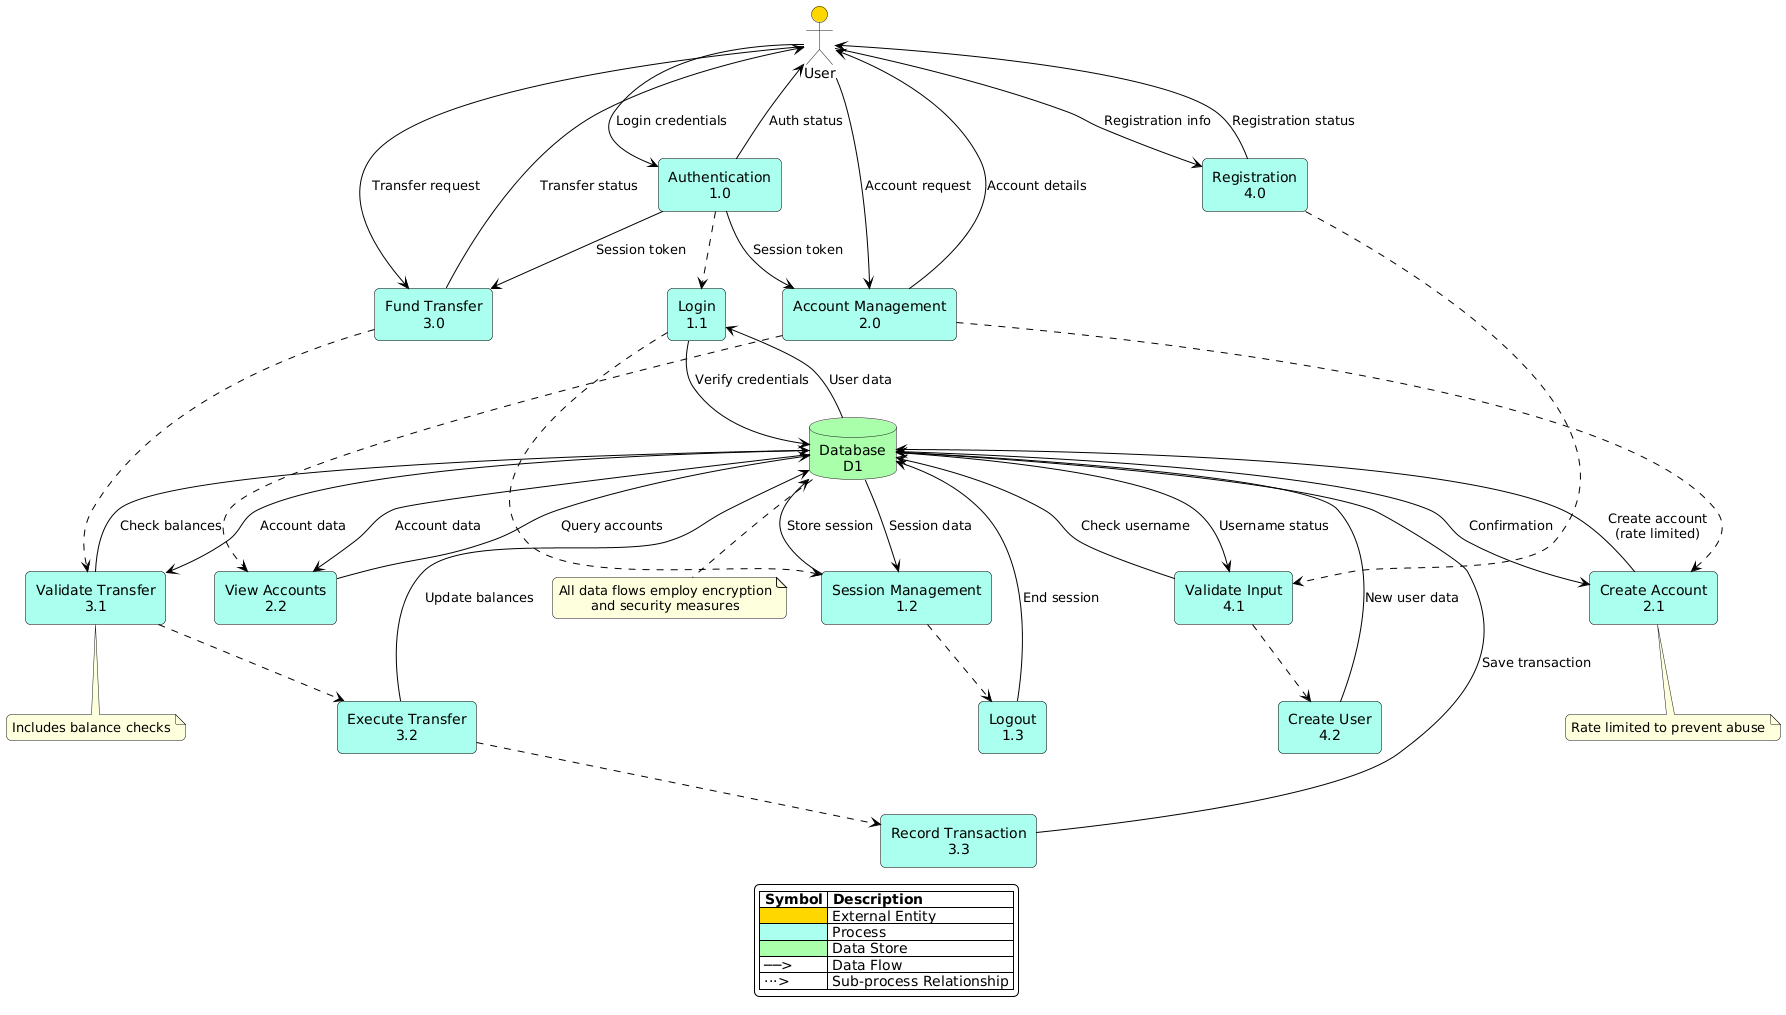
\includegraphics[width=0.8\textwidth, height=0.7\textheight, angle=90]{dataflow.png}

\chapter{Outputs}

\begin{figure}[h]
    \centering
    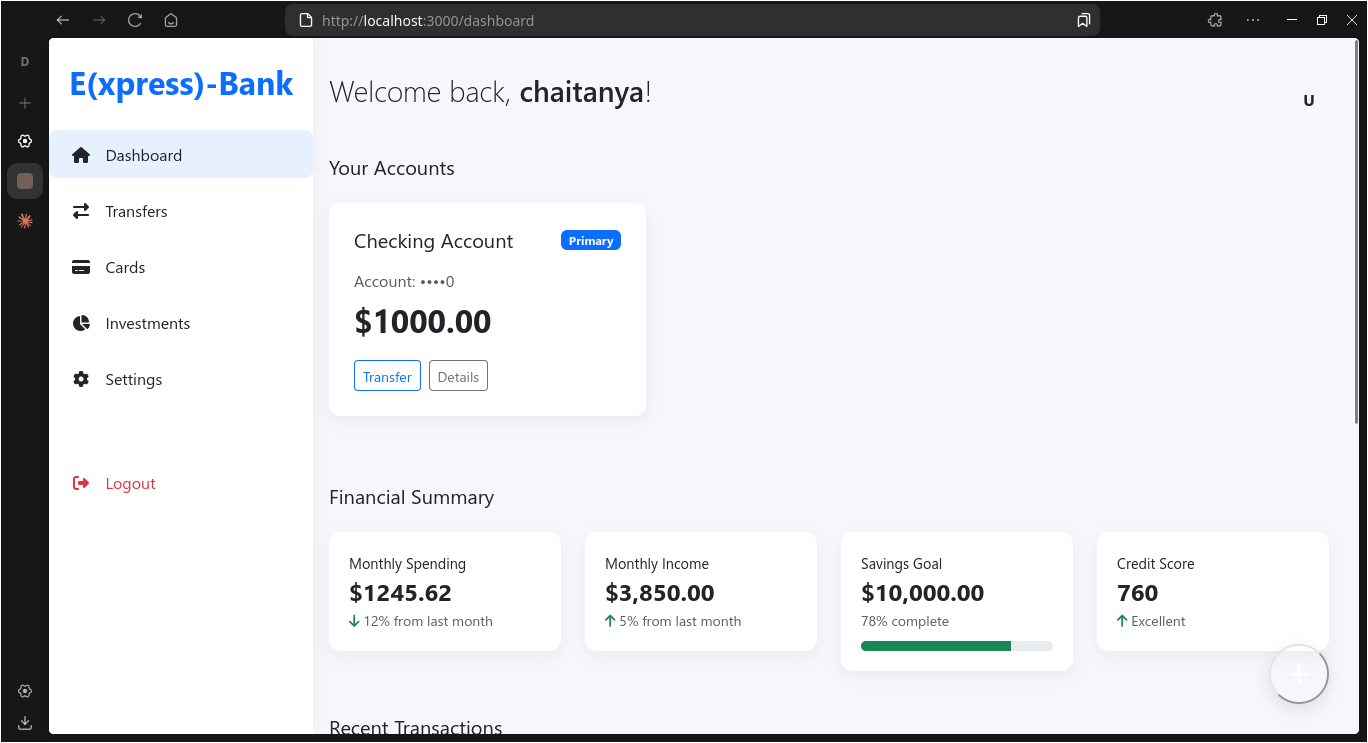
\includegraphics[width=0.8\textwidth]{dashboard.png}
    \caption{Dashboard Interface}
\end{figure}

\begin{figure}[h]
    \centering
    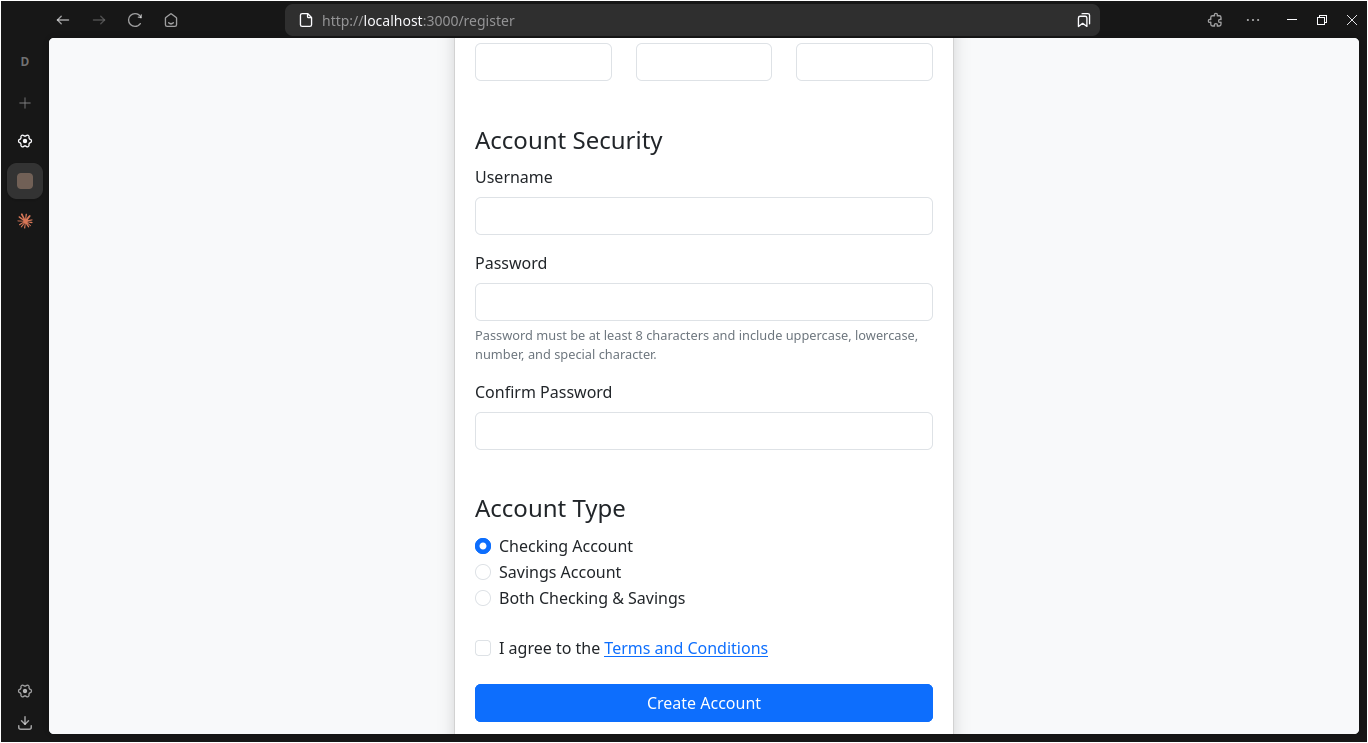
\includegraphics[width=0.8\textwidth]{register.png}
    \caption{User Sign Up Interface}
\end{figure}

\begin{figure}[h]
    \centering
    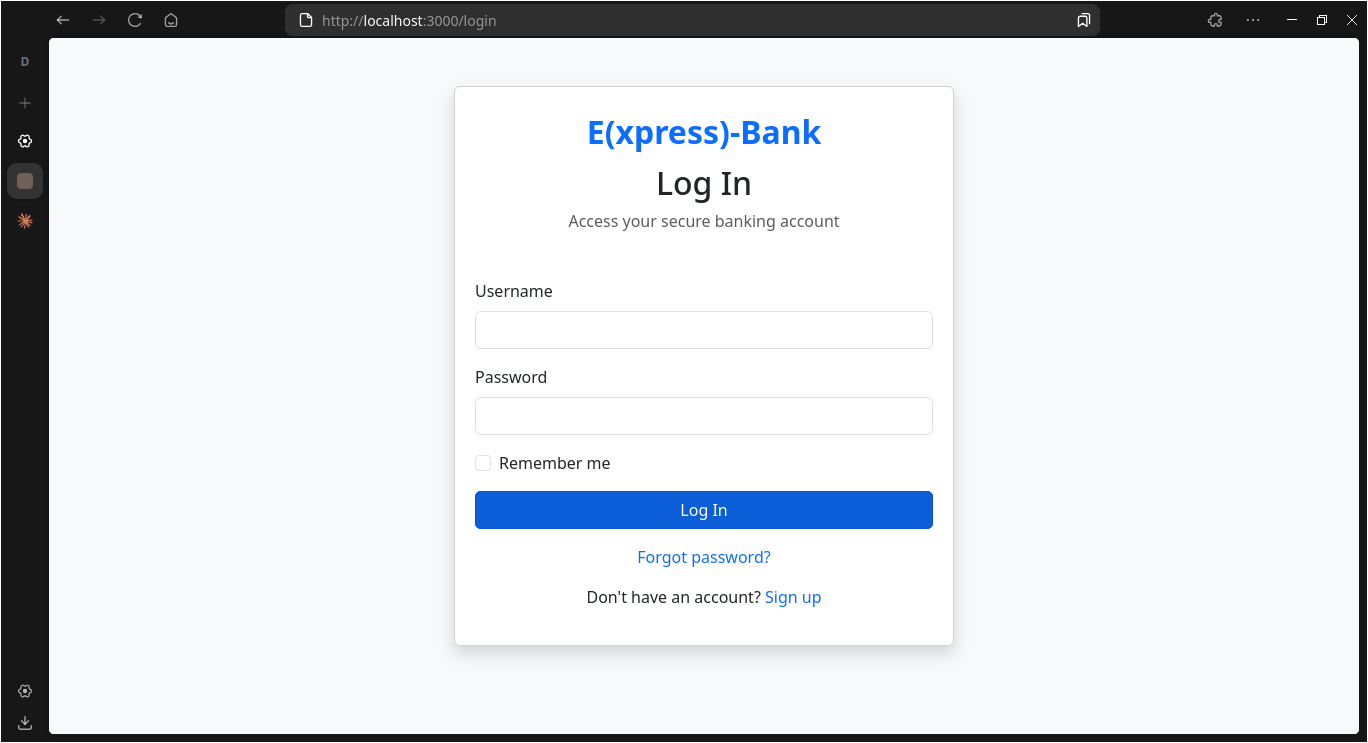
\includegraphics[width=0.8\textwidth]{login.png}
    \caption{User Account Login Interface}
\end{figure}

\begin{figure}[h]
    \centering
    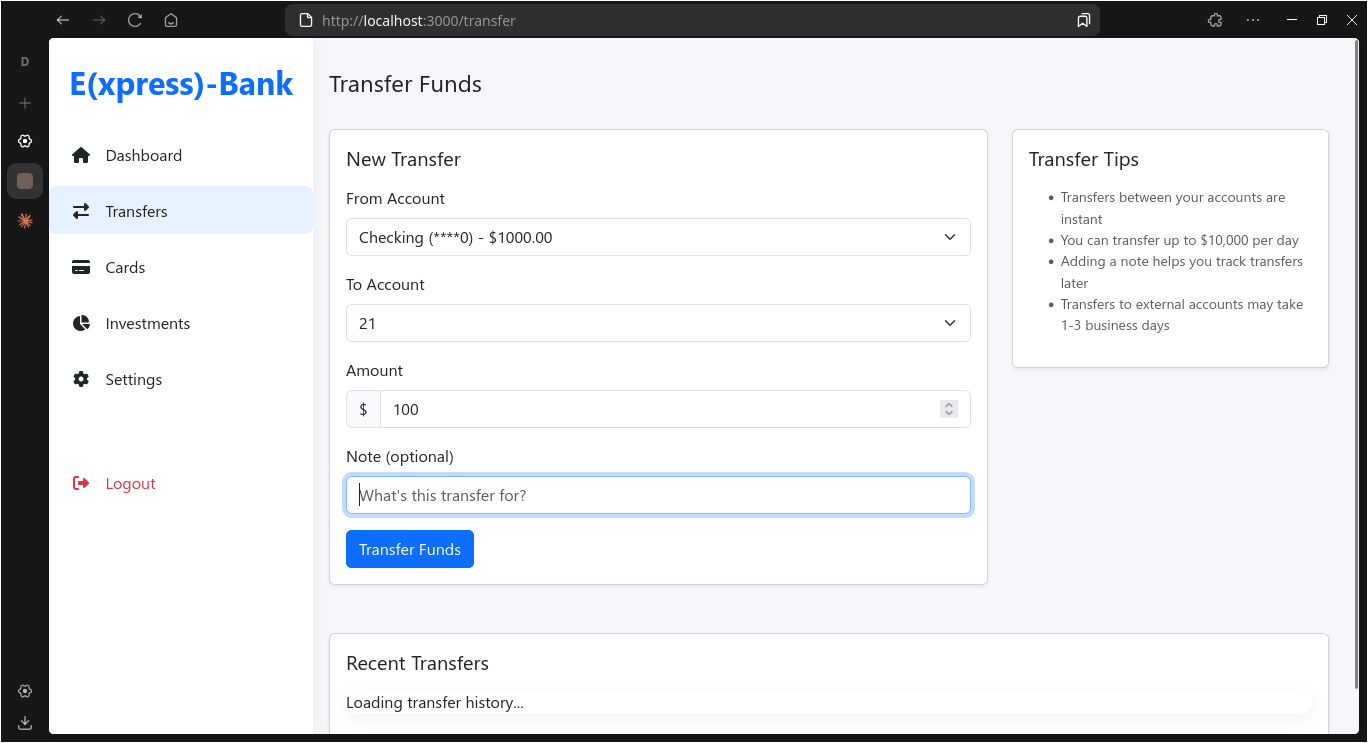
\includegraphics[width=0.8\textwidth]{transfers.png}
    \caption{Transaction Interface}
\end{figure}

\begin{figure}[h]
    \centering
    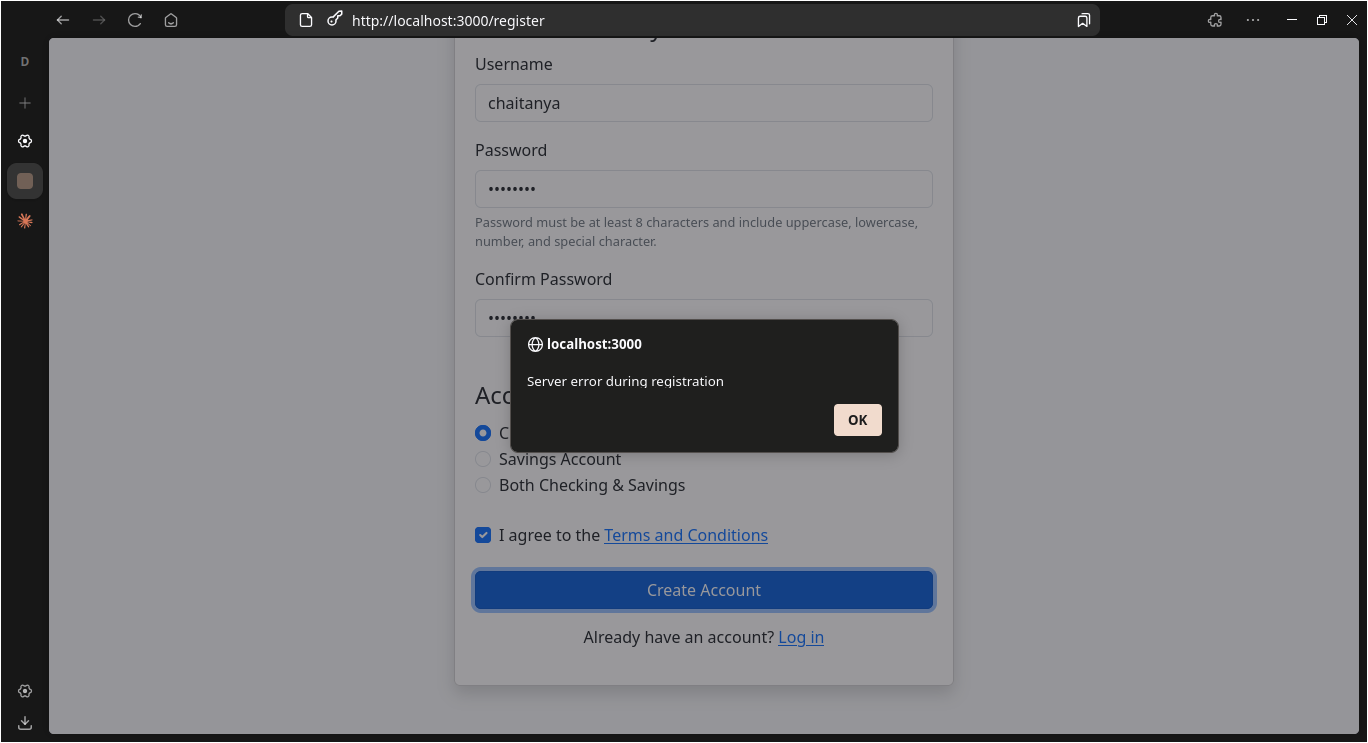
\includegraphics[width=0.8\textwidth]{error.png}
    \caption{Error Messages}
\end{figure}

\chapter{References}

\begin{enumerate}
    \item \raggedright \url{https://stackoverflow.com/questions/5132923/how-to-add-a-primary-key-to-a-mysql-table}
    \item \raggedright \url{https://stackoverflow.com/questions/9070764/insert-auto-increment-primary-key-to-existing-table}
    \item \raggedright \url{https://stackoverflow.com/questions/5813771/in-ejs-template-engine-how-do-i-include-a-footer}
    \item \raggedright \url{https://stackoverflow.com/questions/22212440/using-math-class-to-convert-cosine-into-degrees}
    \item \raggedright \url{https://www.geeksforgeeks.org/how-to-connect-node-js-application-to-mysql/}
    \item \raggedright \url{https://stackoverflow.com/questions/13396119/how-to-add-a-value-to-existing-value-using-sql-query}
    \item \raggedright \url{https://stackoverflow.blog/css/}
\end{enumerate}

\begin{thebibliography}{9}
    \bibitem{Project}
    Full Project Source Code: \textit{https://github/Atan-D-RP4/wt\_project}

    \bibitem{Git}
    Git: \textit{https://git-scm.com/}

    \bibitem{GitHub}
    GitHub: \textit{htps://github.com/}

    \bibitem{Deno}
    Deno: \textit{https://deno.com/}

    \bibitem{nodejs}
    Node.js: \textit{https://nodejs.org/en/}

    \bibitem{bootstrap}
    Bootstrap: \textit{https://getbootstrap.com/}

    \bibitem{express}
    Express.js: \textit{https://expressjs.com/}

    \bibitem{ejs}
    EJS; \textit{https://ejs.co/}

    \bibitem{mysql}
    MySQL: \textit{https://www.mysql.com/}

    \bibitem{visualstudio}
    Visual Studio Code. \textit{https://code.visualstudio.com/}
\end{thebibliography}

\end{document}
